\newpage
\section{Test of the delay Effect}
In this part, tests for the delay effect that show whether it fulfills the requirements are presented. 


\subsection{Test of \autoref{req:delay1}}
According to \autoref{req:delay1}, a test was made to ensure that the delay effect have the specified delays. The test is made by sending a single known sine impulse into the delay effect. The test setup is shown in \autoref{chap:effect_test_response}. The output of the test is plotted in MATLAB and the result is as following \autoref{fig:tests:delay:1kHz}

\begin{figure}[htbp!]
    \centering
        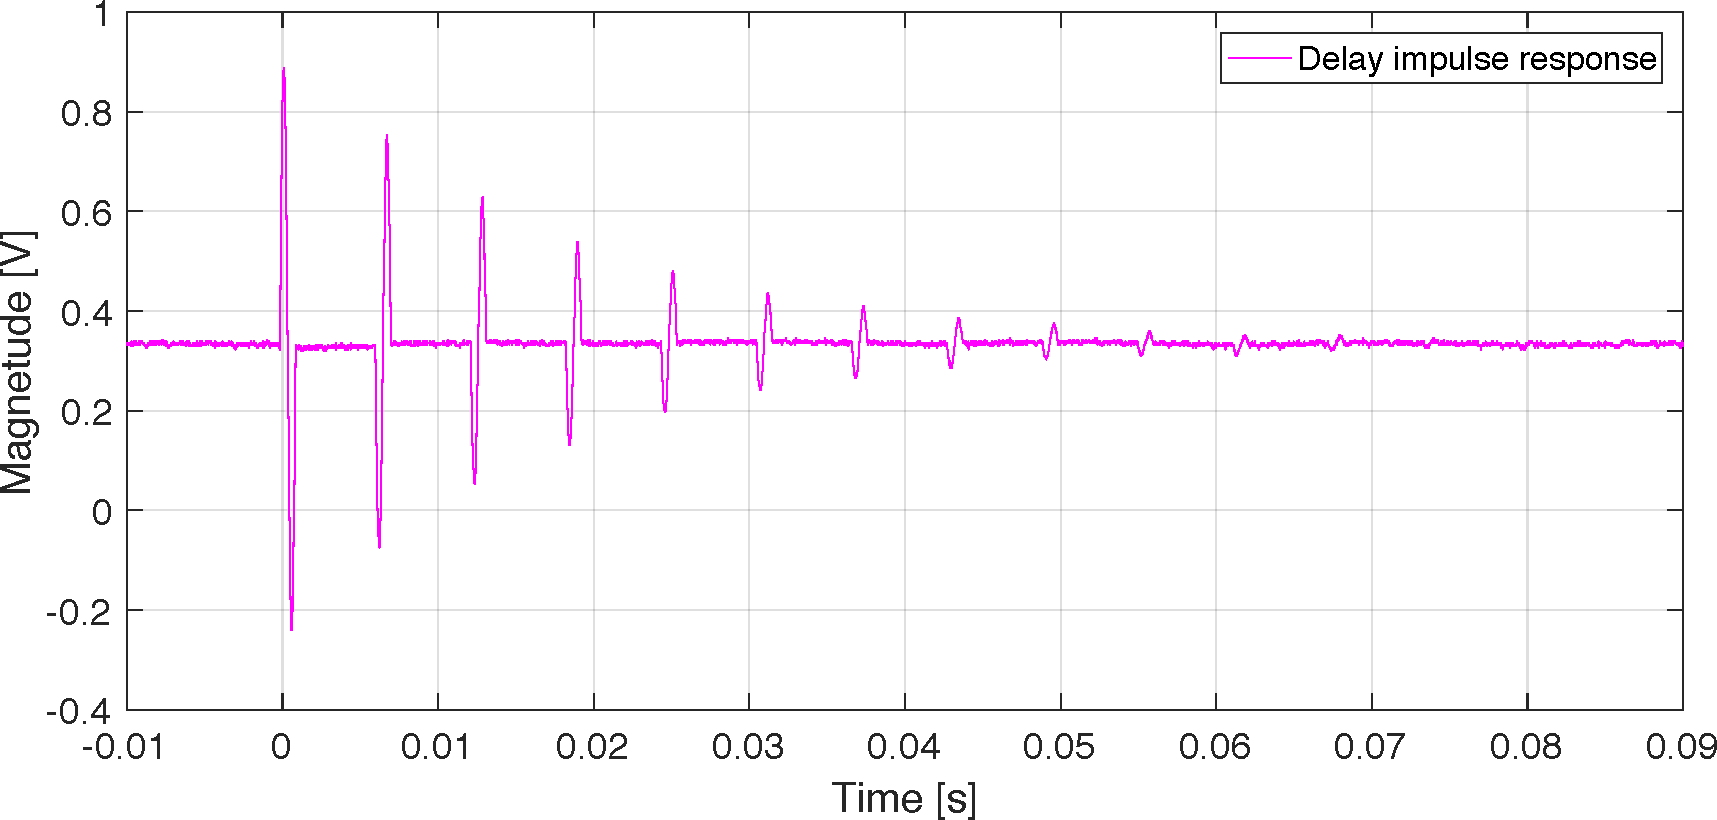
\includegraphics[width=\textwidth]{delay_impulse_response.pdf}
        \caption{Plot of the measured delay impulse response at \SI{1}{\kilo\hertz}.}
        \label{fig:tests:delay:1kHz}
  \end{figure}

Thus the requirement is approved.

\subsection{Test of \autoref{req:delay2}}
Since the user interface not is implemented, \autoref{req:delay2} is conditionally approved because the option is made available in the program.



\subsection{Test review of the delay Effect}
In this subsection, a short review will be shown of the delay effect test.

\begin{table}[H]
\centering
\caption{Recap of the requirements fulfilments for the delay }
\label{test_of_delay_table}
\begin{tabular}{|l|l|}
\hline
\rowcolor[HTML]{9B9B9B} 
\textbf{Requirement} & \textbf{Fulfilment State} \\ \hline
\textbf{\ref{req:delay1}}    & \cmark                     \\ \hline
\textbf{\ref{req:delay2}}    & \cmark*                     \\ \hline
\end{tabular}
\end{table}
